\section{Temporal Replication and Mining}
\label{sec:trm_solution}
The idea of \emph{Temporal Replication and Mining} (TRM)
is to group temporally contiguous snapshots together, s.t. patterns can be
mined from each group of snapshots. In order to achieve the \emph{completeness}
and \emph{soundness} during partitioning, we allow replication of
snapshots among groups. The TRM is outlined in Algorithm~\ref{algo:trm_overview}.

\begin{algorithm}
\caption{Temporal Replication and Mining}
\label{algo:trm_overview}
\begin{algorithmic}[1]
\Require list of $\langle t, S_t \rangle$ pairs
\State {---Map Phase---}
\label{code:trm-map-start}
\ForAll{$\langle t, S_t \rangle$}
	\ForAll{$i \in 1...(K-1)*G+K$}
		\State emit a $\langle t-i, S_t \rangle$ pair
	\EndFor 
\EndFor
\label{code:trm-map-end}
\State {---Partition and Shuffle Phase---}
\label{code:trm-par-start}
\ForAll{$\langle t, S \rangle$ pair} 
\State group-by $t$, emit a $\langle t, Par_t\rangle$,
\State  where $Par_t = \{S_t, S_{t+1}, .. S_{t+(\lceil \frac{K}{L} \rceil -1)*G+2K}\} $
\EndFor
\label{code:trm-par-end}
\State {---Reduce Phase---}
\label{code:trm-red-start}
\ForAll{$\langle t,Par_t \rangle$}
\State lineSweepMining($Par_t$)
\label{code:trm-red-end}
\EndFor
\end{algorithmic}
\end{algorithm}

As shown in Algorithm~\ref{algo:trm_overview}, the TRM algorithm contains
three steps. First, in the map phase, each snapshot is keyed 
with its timestamp (lines~\ref{code:trm-map-start}-\ref{code:trm-map-end}). 
Second, in the partition phase, every snapshot is grouped with its next 
$(\lceil \frac{K}{L} \rceil -1)*G+2K$ snapshots to form a partition (lines~\ref{code:trm-par-start}-\ref{code:trm-par-end}). We will shortly discuss how the group size is derived. 
Third, in the reduce phase, a lineSweepMining method is invoked 
to mine GCMP within each partition (lines~\ref{code:trm-red-start}-\ref{code:trm-red-end}). 
It is easy to see that this method replicates a snapshots 
at most $(\lceil \frac{K}{L} \rceil -1)*G+2K$ times.

\subsubsection{Temporal Replication Partition}
The size of replication is critical for the performance of TRM algorithm.
If the size of replication is too large, the shuffle cost as well as the reduce cost would be high. 
On the contrary, if the size of replication is too small, the \emph{completeness} and \emph{soundness}
properties cannot be satisfied. In the Algorithm~\ref{algo:trm_overview}, 
the partition size is chosen as $(\lceil \frac{K}{L} \rceil -1)*G+2K$. As stated in the following
theorem, such a partition method is sound and complete.
\begin{theorem}[Soundness and Completeness of Replication]
\label{thm:replication_partition}
Let $\mathbb{P}$ be as follows: for each snapshot $S_t$, create a partition $Par_t = \{S_t, ...,S_{t+(\lceil \frac{K}{L} \rceil - 1) *G+2K}\}$. Then $\mathbb{P}$ is sound and complete.
\end{theorem}
\begin{proof}
The soundness of partition can be observed from the fact that each partition represents partial trajectories with consecutive snapshots, therefore patterns in a partition can be directly mapped back to original trajectories.
Given a valid pattern $P$, let $T' \subseteq P.T$ be the subsequence of $P.T$ which conforms to $K,L,G$ with the smallest size. Note that there could be many qualified $T'$s.  
Let the $i^{th}$ local-consecutive part of $T'$ be $l_i$ and let the $i^{th}$ gap of $T'$ be $g_i$. Then, the size of $T'$ can be written as $\Sigma_i (l_i + g_i)$. 
Since $T'$ conforms to $K,L,G$, then $2K \geq \Sigma_i (l_i) \geq K$, $l_i \geq L$, $g_i \leq G$. Therefore, $\Sigma_i(l_i+g_i) \leq (\lceil \frac{K}{L} \rceil -1) *G+2K$. Thus ensuring each $Par_t$ to be of that size would capture at least one of the $T'$s, therefore the pattern $P$ would be valid in $Par_t$. This proves the completeness of the partitioning method.
\end{proof}

\subsubsection{Line Sweep Mining}
After partition, each task in the reduce phase processes a partition $Par_i$, which contains
$(\lceil \frac{K}{L} \rceil -1) *G+2K$ snapshots starting from snapshot $S_i$. With such a 
partition method, we observe that within $Par_i$, only the 
patterns whose object sets are contained in the first snapshot are necessary to be reported.
Therefore, we design a simple \emph{line-sweep mining}(LSM) method for discover
GCMPs. The algorithm works as in Algorithm~\ref{algo:line-sweep}.

\begin{algorithm}
\caption{Line Sweep Mining}
\label{algo:line-sweep}
\begin{algorithmic}[1]
\Require $Par_t = \{S_t, S_{t+1}, ...\}$
\State{$C \gets \{\}$} \Comment{Candidate set} \label{code:ls-can-set}
\For{$c \in S_t$} 
\label{code:ls-init-start}
\State $C$.add($\langle c, t \rangle $)
\EndFor
\label{code:ls-init-end}
\For{$i=1; i < |Par_t|;i++$}
\State $N \gets S_i \oplus C$ \label{code:ls-join}
	\ForAll {$n \in N$}
		\If{$|n.O| \geq M$}
			$C$.add($n$).
			\label{code:ls-add}
		\EndIf
	\EndFor
\State{remove unqualified candidate from $C$}
	\label{code:ls-remove}
\EndFor
\State{output qualified candidate in $C$}
\end{algorithmic}
\end{algorithm}

The algorithm scans the snapshots in a partition in sequential order. During the scan, it
maintains a candidate set $C$ which could potentially be a valid pattern (line~\ref{code:ls-can-set}).
The algorithm starts by inserting clusters at $S_1$ to $C$ (lines~\ref{code:ls-init-start}-\ref{code:ls-init-end}).
Subsequently, in each iteration, clusters in $C$ are joined with clusters at $S_i$ to generate
a new set of patterns $N$(lines~\ref{code:ls-join}). Any valid new patterns are inserted back to $C$
and any invalid patterns are discarded(lines~\ref{code:ls-add} and~\ref{code:ls-remove}).

\begin{figure}[h]
\centering
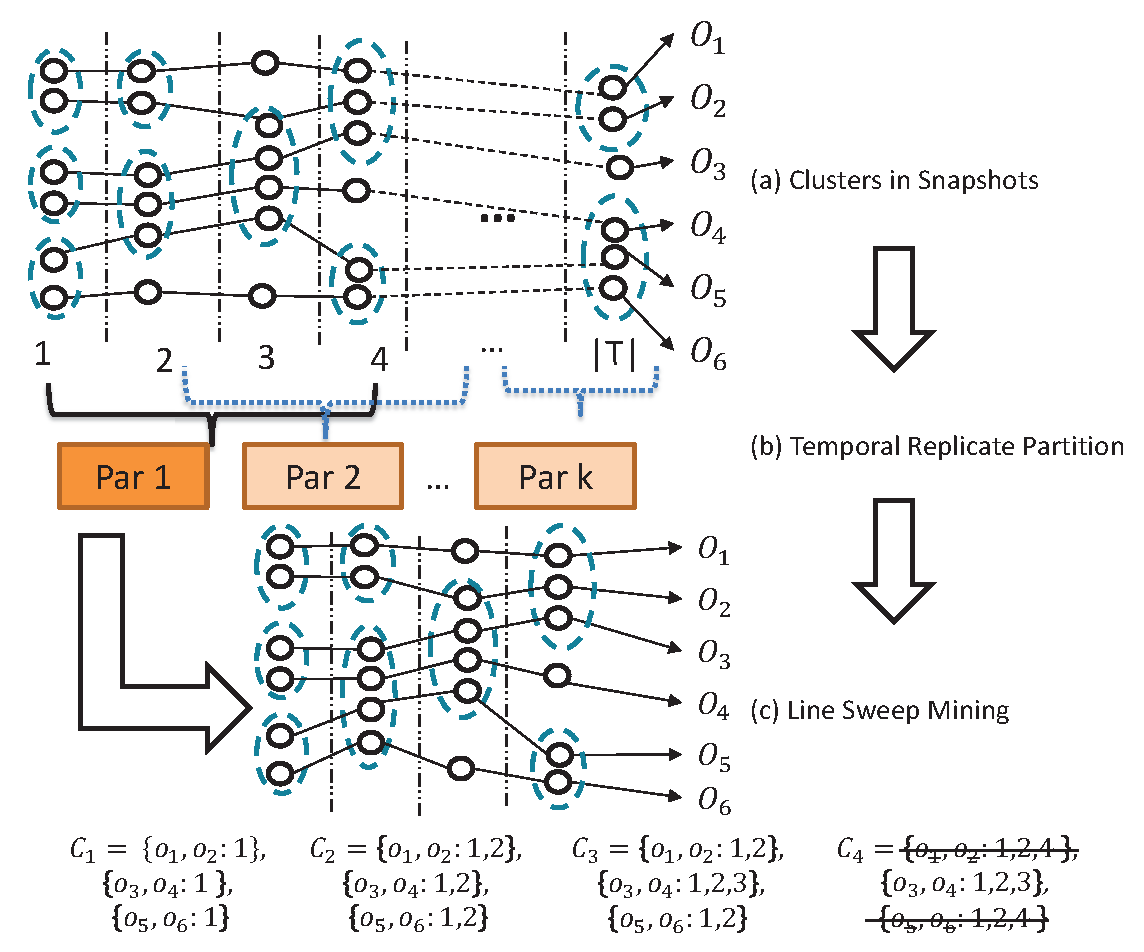
\includegraphics[width=0.5\textwidth]{trm_process.eps}
\caption{Work flow of trajectory replication and mining}
\label{fig:trm_process}
\end{figure}

\begin{example}
We illustrate the process of TRM in Figure~\ref{fig:trm_process} using $M=2, K=2, L = 2, G=2$. In (a), snapshots are clustered and these snapshots are the input to the TRM. Then, we compute the size 
for each partition, which equals to $(\lceil \frac{K}{L} \rceil-1) *G+2K = 4$. Therefore, in (b), every four snapshots
are grouped into a partition. Then a line sweep method is performed in (c) for partition 1. Each
$C_i$ refers to the candidate set  when the algorithm sweeps each snapshot. Initially, $C_1$ contains
patterns whose object set is in $S_1$. When scanning the snapshots, patterns in $C_1$ grow
their timestamps. At $S_4$, since the timestamps of $\{o_1,o_2\}$ and $\{o_5,o_6\}$ 
are both $\{1,2,4\}$ which is neither a qualified set of timestamps nor matches $G$ constraint, 
thus the two candidates are removed from $C_4$. After all snapshots are scanned, 
only $\{o_3,o_4\}$ is the qualified pattern and is outputted.
\end{example}


The TRM approach though achieves good parallelism, 
it requires to replicate the data multiple times. 
Specifically, each snapshots are copied $(\lceil \frac{K}{L} \rceil -1) *G+2K$ times. 
In the cases of \emph{swarm}, \emph{group} and \emph{platoon}, $G$ is as large as $|T|$. 
Handling those cases is equivalent to replicate the entire snapshots to each partition, 
which surrenders the benefit of parallelism.

